\documentclass[a4paper,11pt, oneside]{phdthesis}
%
% for customizing the page size
\usepackage[vcentering,dvips]{geometry}
\geometry{papersize={190mm,260mm},margin=2.5cm, bottom=2.5cm, top=2.5cm}
%
%using fancy header for customizing the page header
\usepackage{fancyhdr}
\pagestyle{fancy}
\fancyhf{}
%
\renewcommand{\chaptermark}[1]{\markboth{\MakeUppercase{#1}}{}}
\renewcommand{\sectionmark}[1]{\markright{\MakeUppercase{#1}}{}}
\renewcommand{\headrulewidth}{3.0pt}
%
\mainmatter{}
\fancyhead[RE,LO]{{\footnotesize\rightmark} }
\renewcommand{\headrulewidth}{0.5pt}
%
\setlength{\headsep}{20pt}
%\setlength{\parskip}{.6cm}
\renewcommand{\baselinestretch}{1.5}
%
\usepackage{color}
\usepackage{graphicx}
\usepackage{latexsym}
\usepackage[tight,footnotesize]{subfigure}
\usepackage{fancyhdr}                    % Fancy Header and Footer 
\usepackage{multirow}
\usepackage{longtable} 
\usepackage{comment}
\usepackage{algorithmic}
\usepackage{multirow}

%\usepackage{algorithm}
\usepackage{tipa}
\usepackage[ruled,lined,commentsnumbered]{algorithm2e}
\usepackage[ruled,lined,commentsnumbered]{algorithm2e}
%\usepackage{setspace}
%\usepackage{txfonts}
%\usepackage{algorithmicx}
%\usepackage{algpseudocode}
\usepackage{cite}
\DeclareGraphicsExtensions{.eps}
\usepackage[fleqn]{amsmath}
\DeclareMathOperator*{\argmax}{arg\,max}
\usepackage{amssymb}
\usepackage{titletoc}

%from here
%\usepackage{fontspec}
%
%\usepackage{polyglossia}
%
%%\setmainfont{[Kalpurush.ttf]}
%\setmainfont{[Siyamrupali.ttf]}

%\setmainfont{FreeSerif:script=Kalpurush.ttf}

%to here

%\usepackage{polyglossia}
%\setmainlanguage[numerals=Devanagari]{bengali}
%\setotherlanguage{english}
%\newfontfamily\englishfont[Scale=MatchLowercase]{Linux Biolinum O}
%\newfontfamily\bengalifont[Script=Bengali]{Akaash}



%\usepackage{amsfonts,amssymb, txfonts, dsfont}
%\usepackage{amsmath,amsthm,txfonts}
%changing the font
%\usepackage{mathptmx}
%\usepackage{pslatex}
%\usepackage{palatino}
\newtheorem{definition}{Definition}
\newtheorem{mypro}{Property}
\newtheorem{proposition}{Proposition}
\newtheorem{proof}{Proof}
\newtheorem{corollary}{Corollary}
\newtheorem{theorem}{Theorem}
\newtheorem{lemma}{Lemma}

%
% following commands add the word chapter in table of contents
\makeatletter 
\newcommand*\stdl@chapter{} 
\let\stdl@chapter\l@chapter 
\newcommand*\realchapter{% 
  \renewcommand*\l@chapter[2]{% 
    \stdl@chapter{\chaptername\space##1}{##2}}} 
\newcommand*\fakechapter{\let\l@chapter\stdl@chapter} 
\makeatother 
\newcommand*\switchchapter[1]{\addtocontents{toc}{\expandafter\protect\csname #1chapter\endcsname}}
%
\newenvironment{xlist}[1]{%
\begin{list}{}{%
    \settowidth{\labelwidth}{#1}
    \setlength{\labelsep}{0.5cm}
    \setlength{\leftmargin}{\labelwidth}
    \addtolength{\leftmargin}{\labelsep}
    \setlength{\rightmargin}{0pt}
    \setlength{\parsep}{0.5ex plus0.2ex minus0.1ex}
    \setlength{\itemsep}{0ex plus0.2ex}
    }
  }
{\end{list}}
%
\definecolor{MyBlack}{cmyk}{1,1,1,1}
\color{MyBlack}
%\color{black}
%
\begin{document}

\include{Cover}
\begin{titlepage}
\begin{center}
%
\vspace*{0.5cm}
%
\noindent{\large \textbf{Thesis for the Degree of B.Sc. Engineering}}\\
\vspace*{1.2cm}
%
%\noindent{\LARGE \textbf{{\fontfamily{ptm}\selectfont Path selection and channel access for IEEE 802.11s Wireless Mesh Network}}}\\
%
%\noindent{\LARGE \textbf{{\fontfamily{ptm}\selectfont High performance extensions of IEEE 802.11s standardization for Wireless Mesh Networks}}}\\
%
\noindent{\LARGE \textbf{{\fontfamily{ptm}\selectfont Thesis Title}}}\\

%\noindent{\LARGE \textbf{{\fontfamily{ptm}\selectfont Enhanced channel access and path selection for IEEE 802.11s Wireless Mesh Networks}}}\\
%
\vspace*{4.0cm}
\noindent \LARGE \textbf{Author Name} \\[-15pt]
\noindent \LARGE \textbf{Student ID: 20111...} \\
%
\vspace*{4.5cm}
%
\noindent{\large \textbf{Department of Computer Science and Engineering}}  \\[-15pt]
\noindent{\large \textbf{Bangabandhu Sheikh Mujibur Rahman Science and Technology}}\\[-15pt]
\noindent{\large \textbf{University, Gopalganj, Bangladesh}}\\[-15pt]

\vspace{1.5cm}
\noindent{\large \textbf{December, 2015}}
%
\end{center}
\end{titlepage}
\sloppy
%
\titlepage
%

\begin{titlepage}
\begin{center}
%
%\vspace*{0.30cm}
%
%\noindent{\large \textbf{Thesis for the Degree of Master of Science}}\\
%
%\noindent{\huge \textbf{{\fontfamily{ptm}\selectfont Thesis for the Degree of Master of Science}}}\\[5pt]
%\vspace*{0.75cm}
\noindent{\LARGE \textbf{{\fontfamily{ptm}\selectfont Thesis Title }}}\\
%
%\noindent \Huge \textbf{P H D\ \ T H E S I S} \\
\vspace*{1cm}
\noindent \large \textbf{by} \\[-7pt]
\noindent \Large \textbf{Author Name} \\
\noindent \Large \textbf{Student ID: } \\
%
\vspace*{1cm}
\noindent \large \textbf{Supervised by} \\[-7pt]
\noindent \Large \textbf{Supervisor Name } \\
%
\vspace*{1cm}
%
\noindent{\large \textbf{Submitted to the Department of Computer Science and }}  \\[-11pt]
\noindent{\large \textbf{Engineering of Bangabandhu Sheikh Mujibur Rahman Science }}  \\[-11pt]
\noindent{\large \textbf{and Technology University in partial fulfillment of the }}  \\[-11pt]
\noindent{\large \textbf{ requirements for the degree of B.Sc. Engineering}}  \\[-11pt]
\noindent{\large \textbf{}}\\[-11pt]
%\noindent{\large \textbf{Kyung Hee University in partial fulfillment}}\\[-11pt]
\noindent{\large \textbf{}}\\[-11pt]
\noindent{\large \textbf{}}\\
%
\vspace{3.25cm}
%
\begin{minipage}{5.25in}
\flushleft{\hspace{20pt}\large \textbf{\underline{Thesis Evaluation Committee:}}}  \\[10pt]
\noindent{\hspace{20pt}\large \textbf{Teacher Name 1} $\dots\dots\dots\dots\dots\dots \dots\dots\dots\dots\dots.$}\\[11pt]
\noindent{\hspace{20pt}\large \textbf{Teacher Name 2} $\dots\dots\dots\dots\dots\dots\dots\dots\dots\dots\dots$}  \\[11pt]
\noindent{\hspace{20pt}\large \textbf{Teacher Name 3} $\dots\dots\dots\dots\dots\dots\dots\dots\dots\dots\dots.$} 
\textcolor{white}{nothing}
\end{minipage}
%
% following figure adds the scanned signature of the professor
%
%\begin{figure}[!b]
%\centering
%%\begin{minipage}{4.6in}
%%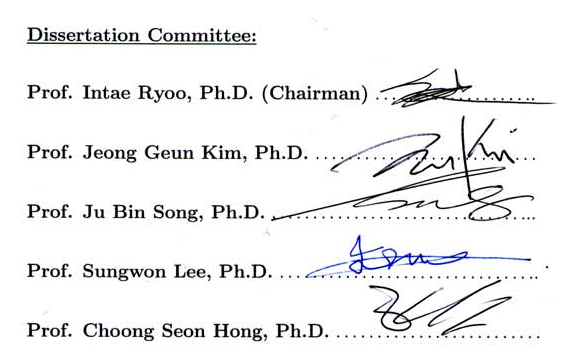
\includegraphics[scale=1.25]{Fig_Thesis_Signature.eps}
%%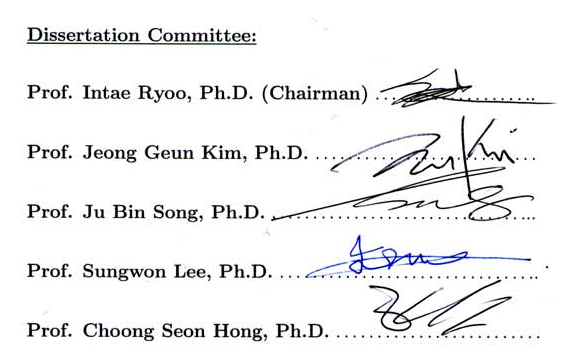
\includegraphics[width=1.62in,height=2.4in]{Fig_Thesis_Signature.eps}
%%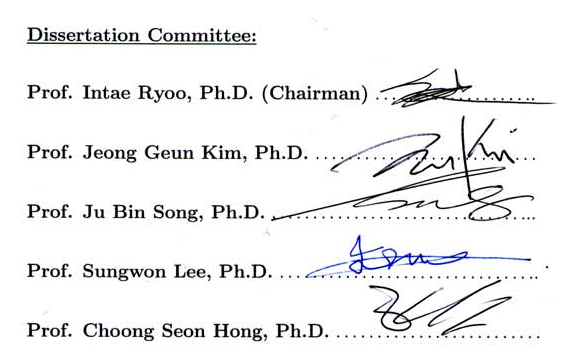
\includegraphics[width=4.5in]{Fig_Thesis_Signature.eps}
%\label{Fig_Thesis_Signature}
%%\end{minipage}
%\end{figure}
%%
\end{center}
\end{titlepage}
\sloppy
%
\titlepage
%

\begin{titlepage}
\begin{center}
%
%\vspace*{0.5cm}
%
\noindent{\LARGE \textbf{Thesis Approval}}\\
%\vspace*{1.2cm}
%
%\noindent{\LARGE \textbf{{\fontfamily{ptm}\selectfont Path selection and channel access for IEEE 802.11s Wireless Mesh Network}}}\\
%
%\noindent{\LARGE \textbf{{\fontfamily{ptm}\selectfont High performance extensions of IEEE 802.11s standardization for Wireless Mesh Networks}}}\\
%
 Student's Name:\\ 
 Student's ID:\\ 
 Thesis Title: :\\ 


%\noindent{\LARGE \textbf{{\fontfamily{ptm}\selectfont Enhanced channel access and path selection for IEEE 802.11s Wireless Mesh Networks}}}\\
%
\vspace*{.5cm}
We the undersigned, recommend that the thesis completed by the student listed\\ [-5pt]
 above, in partial fulfillment of B.Sc. Engineering degree requirements, be accepted \\[-5pt] 
by the Department of Computer Science and Engineering, Bangabandhu Sheikh \\[-5pt]
 Mujibur Rahman Science and Technology for deposit. 

\vspace*{1.0cm}
\noindent \large \textbf{Supervisor Approval*} \\[15pt]
............................. \\ [-5pt]
Name of Supervisor \\ [-5pt]
Designation of Supervisor \\ [-5pt]


\vspace*{1.0cm}
\noindent \large \textbf{Additional Approvals ( if requires)*} \\[15pt]
  ............................. \\ [-5pt]
  Name of Supervisor \\[-5pt]
  Designation of Supervisor \\[-5pt]

\vspace*{1.0cm}
\noindent \large \textbf{Departmental Approval} \\[15pt]
............................. \\ [-5pt]
Name of Head of the Department \\ [-5pt]
Chairman, Department of Computer Science and Engineering \\ [-5pt]
%
%\vspace*{4.5cm}
%\vspace*{1.75cm}
%\noindent \large \textbf{Supervised by} \\[-7pt]
%\noindent \Large \textbf{Prof. Choong Seon Hong, Ph.D.} \\
\vspace*{1.5cm}
\noindent{\large \textbf{Bangabandhu Sheikh Mujibur Rahman Science and Technology}}\\
\noindent{\large \textbf{University, Gopalganj, Bangladesh}}\\[-15pt]


%
\end{center}
\end{titlepage}
\sloppy
%
\titlepage
%

\begin{titlepage}
\begin{center}
%
\vspace*{0.5cm}
%
\noindent{\large \textbf{\textcolor{white}{Thesis for the B.Sc Engineering}}}\\
\vspace*{1.2cm}
%
\vspace*{5.5cm}
%
%\noindent \large \emph{\textbf{To my parents and my wife}} \\
\noindent \large \emph{\textbf{Dedicated to my parents, Mr. A  \\
And \\
Mrs. B}} \\
%
\vspace*{4.5cm}
%
\end{center}
\end{titlepage}
\sloppy
%
\titlepage
%


%
%: ----------------------- abstract ------------------------
%
% Your institution may have specific regulations if you need an abstract and where it is to be placed in the document. The default here is just after title.
%
\frontmatter{}
%
% adding the abstract 
% this also adds the abstract in the table of contents
\fancyhead[RO, RE]{\thepage}
\setcounter{tocdepth}{2}
%
\switchchapter{fake} 
\addcontentsline{toc}{chapter}{Abstract}
%
% Thesis Abstract -----------------------------------------------------
%
% -------------------------------------------------------------------- 
%\pagenumbering{roman} \setcounter{page}{1} 
%\noindent{\large  \textbf{{\fontfamily{ptm}\selectfont Supergraph based Periodic Behavior Mining in Dynamic Networks}}}\\
%by \\
%Sajal Halder  


\chapter*{Abstract\markboth{Abstract}{Abstract}}

Bengali is one of the ten most spoken languages in the world, with almost 200 million speakers. Growing online resources reveal a clear need for Bengali language applications and retrieval systems. The development of the internet, there are huge number of Bangla news articles are published every day on the web from different sources and this amount is growing rapidly day by day. Therefore, people have not enough time to read each document with a specified time limit. Bangla document ranking handles this difficulty with an efficient manner. Although, there are more works have been done in English and other European languages, but there is no contribution are present in bangla language to rank a document.  In our thesis, we rank bangla document using term frequency and cosine similarity. We take document as vector and query as vector. We measure term frequency each word in each document. Then finding out score using cosine similarity. Then sorted the scores and ranked the documents. We demonstrate the effectiveness of the technique for bangla document ranking.


%
% adding the acknowledgment 
% this also adds the acknowledgment in the table of contents
\switchchapter{fake} 
\addcontentsline{toc}{chapter}{Acknowledgment}
%
% -------------------------------------------------------------------- 
%\pagenumbering{roman} \setcounter{page}{1} 
\chapter*{Acknowledgment\markboth{Acknowledgment}{Acknowledgment}} 
%\renewcommand{\baselinestretch}{1.2} 
%

At first I like to thank almighty Allah who gives me ability to perform the Thesis. Then I like to give many thanks to my thesis supervisor Md.Nesarul Hoque, Lecturer, Department of Computer Science and Engineering, who encouraged, supervised and supplied necessary requirements and guideline in performing this work. His inspiration for doing research on Bangla Document Ranking by using Term Frequency and Cosine Similarity let me capable to complete the Thesis. I am grateful to him for his unvarying encouragement and simulating ideas. I also like to give thanks to all my teachers and also that of my friends who gave me advice for the completeness of the thesis. Finally I like to special thank to my parents and all my well wishers for their encouragement and support along my study life. 


\vspace{1cm}

\hfill Shraboni Afroz Samapti 

\hfill December, 2016
%

%
%: ----------------------- contents ------------------------
%
\setcounter{secnumdepth}{3} % organisational level that receives a numbers
\setcounter{tocdepth}{3}    % print table of contents for level 3
\switchchapter{fake} 
\renewcommand\contentsname{Table of Contents}
%\addcontentsline{toc}{chapter}{Table of Contents} 
\tableofcontents            % print the table of contents
\cleardoublepage
% levels are: 0 - chapter, 1 - section, 2 - subsection, 3 - subsection
%
%: ----------------------- list of figures ------------------------
\switchchapter{fake} 
%\addcontentsline{toc}{chapter}{List of Figures}
\listoffigures	% print list of figures
\cleardoublepage
%
%: ----------------------- list of tables ------------------------
\switchchapter{fake} 
%\addcontentsline{toc}{chapter}{List of Tables}
\listoftables  % print list of tables
\switchchapter{real}
\newpage
%
%: ----------------------- list of algorithms ------------------------
\switchchapter{fake} 
%\addcontentsline{toc}{chapter}{List of Algorithms}
\listofalgorithms
\switchchapter{real}
%
\mainmatter{}
\fancyhead[RE,LO]{{\thesection}\hspace{0.5em} {\footnotesize\rightmark} }
\renewcommand{\headrulewidth}{0.5pt}
%
% start the arabic page numbering
\pagenumbering{arabic} \setcounter{page}{1} 
%
% now switch to real chapters
%
\chapter{Introduction}
\label{Ch_Chapter1}



\section{Organization of the Thesis}
%
The dissertation is organized as follows: 

\begin{itemize}

\item {•} \textbf{Chapter 1 Introduction.} In this chapter an introduction to the periodic patterns mining researches is presented. The definition, importance and existing approaches are clearly introduced. After that, the dissertation focuses the contribution. 

\item {•} \textbf{Chapter 2 Related Work.} This chapter first shows the state of the art methods of the periodic patterns mining research. Then describe two existing periodic pattern mining works $PSEMiner$ and $ListMiner$ in dynamic networks. The limitations of these methods are clearly addressed, as these are the focuses of this dissertation. 

\item {•} \textbf{Chapter 3 SPBMiner.} We present our proposed technique for mining periodic behaviors in dynamic networks.  

\item {•} \textbf{Chapter 4 Experiments Analysis.} In this chapter, it has been shown the effectiveness and efficiency of our proposed method.

\item {•} \textbf{Chapter 5 Conclusion and Future Work.} Finally, this chapter concludes the dissertation indicating the limitations and future works.
\end{itemize} 
%

\chapter{Related Works}
\label{Ch_Chapter2}
%
%\section{Introduction}
%

\chapter{Proposed System}
\label{Ch_Chapter3}


We have used two methods for ranking document. One is term frequency and another is cosine similarity.

\section{Creating Document Vector}
The process of creating document vector is given below.

\subsection{Term Frequency}

A term that appears many times within a document is likely to be more important than a term that appears only once.\\
D1: {\unicodefont আমি  বাংলাদেশকে ভালবাসি । বাংলাদেশ নদীমাতৃক দেশ।}  \\ 
D2: {\unicodefont আমি বাংলাদেশের নাগরিক । কিন্তু বাংলাদেশের সকল  নাগরিক তাদের মোলিক অধিকার পায় না।} \\
D3: {\unicodefont বাংলাদেশ উন্নয়নশীল দেশ। এখনো উন্নয়নের দিক থেকে পিছিয়ে আছে বাংলাদেশ । } \\

After performing the term frequency calculation we get the table \ref{tab:tab1}. Which is showing the value each word each document.

\begin{table*}[htp]	
\centering

  \caption{Parameters of datasets }
\vspace{0.5cm}
\begin{tabular}{|c|c|c|c|} 
\hline

\textbf{Term} &\textbf{Doc1} 	 & \textbf{Doc2} &\textbf{Doc3}   \\ \hline
{\unicodefont আমি} 		& 1 & 1 &	   \\ \hline
{\unicodefont বাংলাদেশ}	& 2 & 2 & 2   \\ \hline
{\unicodefont ভালবাসি }	& 1 &  &   \\ \hline
{\unicodefont উন্নয়নশীল } 	&  &  &   \\ \hline
{\unicodefont দেশ } 	&  &  & 1  \\ \hline
{\unicodefont নদীমাতৃক }  & 1 &  &   \\ \hline
{\unicodefont কিন্তু}	&  & 2 &   \\ \hline
{\unicodefont সকল}সকল	&  & 1 &   \\ \hline
{\unicodefont মোলিক}	&  & 1 &   \\ \hline
{\unicodefont অধিকার}	&  & 1 &   \\ \hline
{\unicodefont পায়}	&  & 1 &   \\ \hline
{\unicodefont এখনো}	&  &  & 1  \\ \hline
{\unicodefont দিক}  &  &  & 1 \\ \hline
{\unicodefont থেকে} &  &  & 1 \\ \hline
{\unicodefont পিছিয়ে}&  &  & 1 \\ \hline
{\unicodefont আছে}&  &  & 1 \\ \hline
{\unicodefont নাগরিক}&  & 2 &  \\ \hline
{\unicodefont না} &  & 1 &  \\ \hline
{\unicodefont তাদের}&  & 1 &  \\ \hline

\end{tabular}
\label{tab:tab1}
\end{table*}



\subsection{Stop Word Removing}
Documents contain words that do not add information but are necessary for syntactical formation,such as words like {\unicodefont এবং , অথবা , কিন্তু } etc. Since these words are less useful and less informative,  they introduce  noise into the document representation. In order to get rid of these kind of words, a stop word removal step is used.  Stop word removal is done using predefined, human-made list of words. Since a predefined list is used, this approach is language dependent. Instead of using these kinds of lists, a frequency threshold can be used. If a word is seen more\/less frequently than predefined threshold, that word can be considered as stop word. But decision of threshold is another issue to be considered.

\subsection{Stemming}

In a document a word can be seen in different formats, such as plural vs. singular, present vs. past tense, etc. Most of the time these words have the same meaning and treating them differently is unnecessary. In order to use these words as the same token(concept), stemmers are used.
Stremmers are tools that reduce the orginal word forms into roots(stems) of these words. Stemmers are necessary to represent different forms in a single format and to reduce memory usage for storing the words. Also, smaller list of words make it easir to perform calculations. As a result of performing stemming,document representation is less noisy and more dense. The efficiency of a stemmer is important while performing further calculations. In Figure \ref{Figure:stemm} ,we can see the full process of ranking.

Sometimes stemmers can do over-stemming such that two words are given the same stem,while it should not be. For example, the words {\unicodefont “বাংলাদেশের”} and {\unicodefont “বাংলাদেশকে”} are two different words, which should not be stemmed into the same root. But stemmers can find out their root as {\unicodefont “বাংলাদেশ”}. Another steamming problem is related to under stemming such that two words should have been stemmed into the same word, but have not been. for example, {\unicodefont “হাসি”} and {\unicodefont ‘হাসানো’} can be found as two different stems,instead of one.



\subsection{Weighting Term}

Then find weight in a document for each term using the equation \ref{eq:eq1}

\begin{equation}
Weight++=postings[term][doc]*IDF
\label{eq:eq1}
\end{equation}

%\(Weight++=postings[term][doc]*IDF\)

Then assigning document IDS we keep them into database as vector after doing following steps which is shown in Figure \ref{Figure:indexing}.

\subsubsection{Inverse Document Frequency(IDF)}

A term that occurs in a few documents is likely to be a better discriminator than a term that appears in most or all documents.

Then assigning document IDS we keep them into database as vector after doing these steps.


\begin{figure*}[htp]
	\centering
		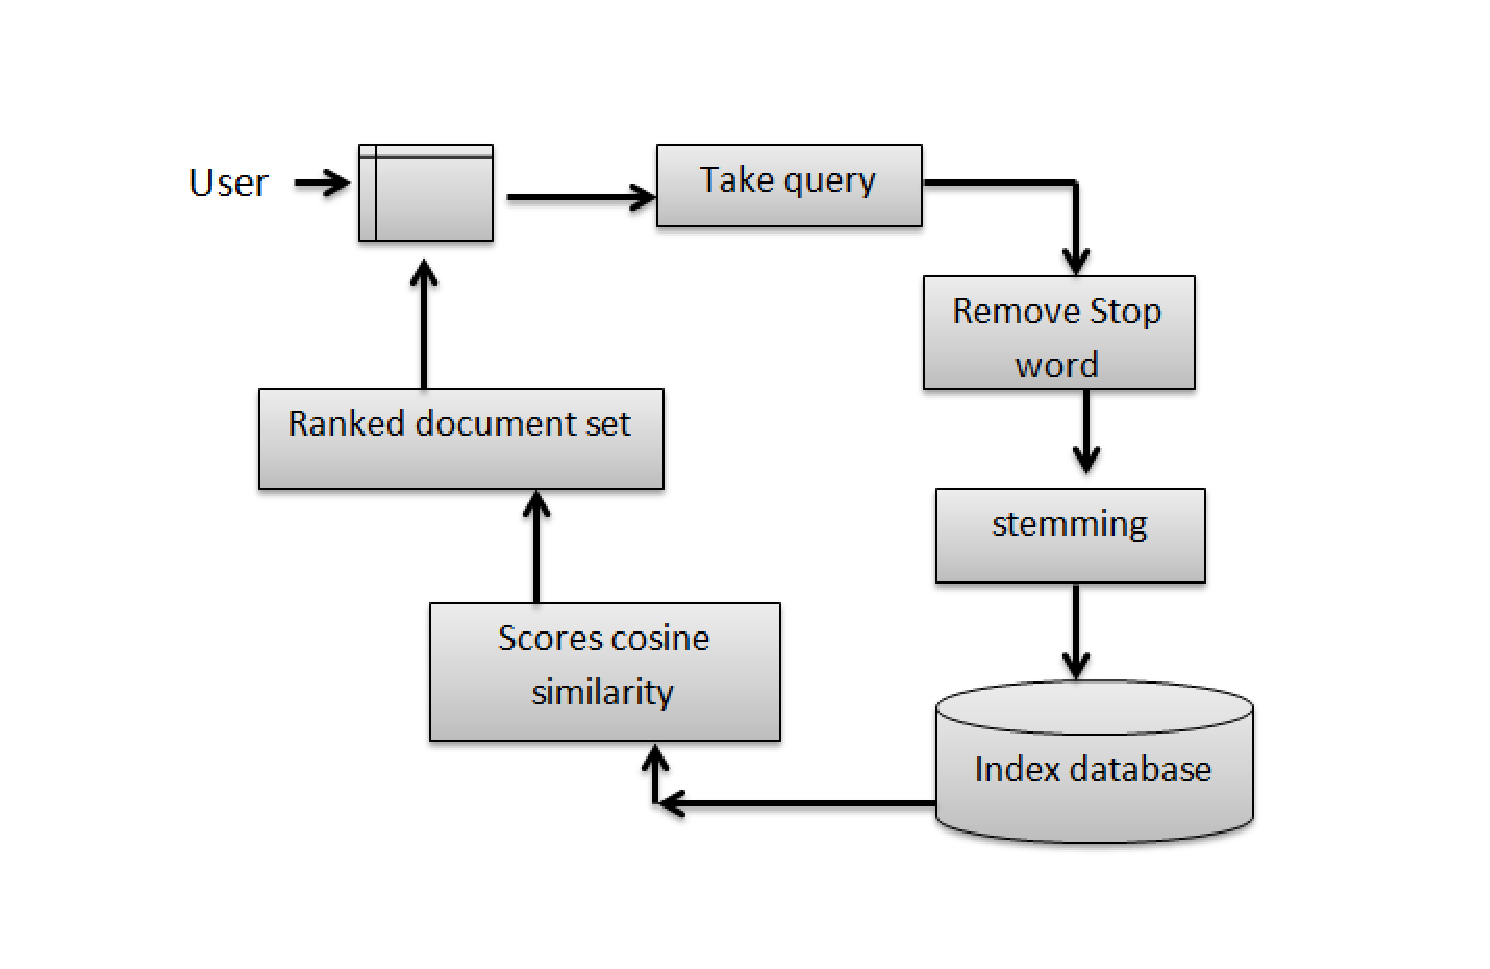
\includegraphics[width=.65\textwidth]{figure/two.eps}
	\caption{Indexing Document Ids \& keep it in a vector.}
	\label{Figure:indexing}
\end{figure*}


\section{Preprocessing of Taking Query}

For taking search query the preprocessing steps have to be done. After taking query step by step process has been done . And then match query with relevent documents. The preprocessing steps are showing in the figure \ref{Figure:inquery} below.


\begin{figure*}[htp]
	\centering
		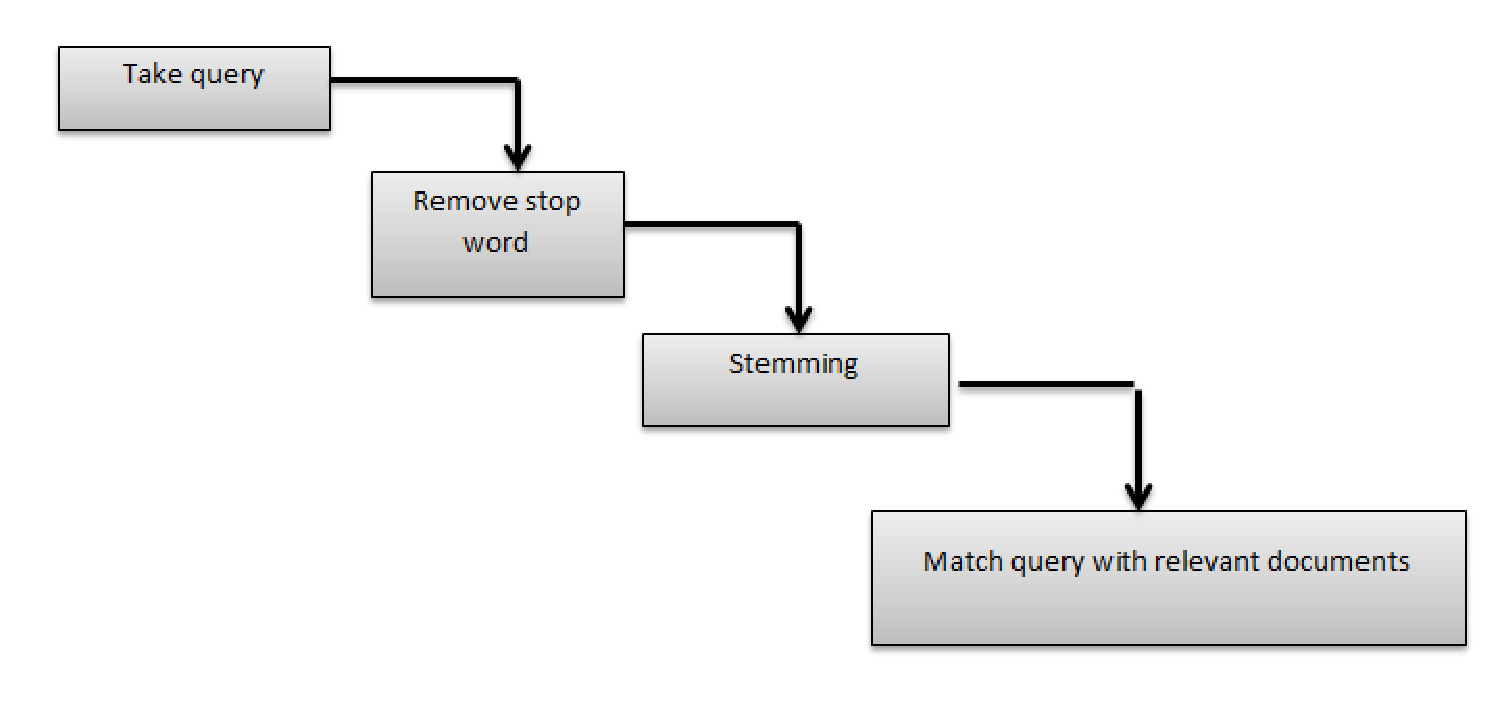
\includegraphics[width=.65\textwidth]{figure/three.eps}
	\caption{Pre processing of Input query}
	\label{Figure:inquery}
\end{figure*}


\subsection{Removal of Stop Word}

The less importance word should be removed from query. Sometimes input query contain words that do not add information, such type words {\unicodefont ‘এবং’ , ‘অথবা’ , ‘কিন্তু ’} etc should remove from document.

\subsection{Stemming}

Finding root words from other similar words which have the same meaning and treating them differently is unnecessary. Figure \ref{Figure:stemm} showing the process.

\begin{figure*}[htp]
	\centering
		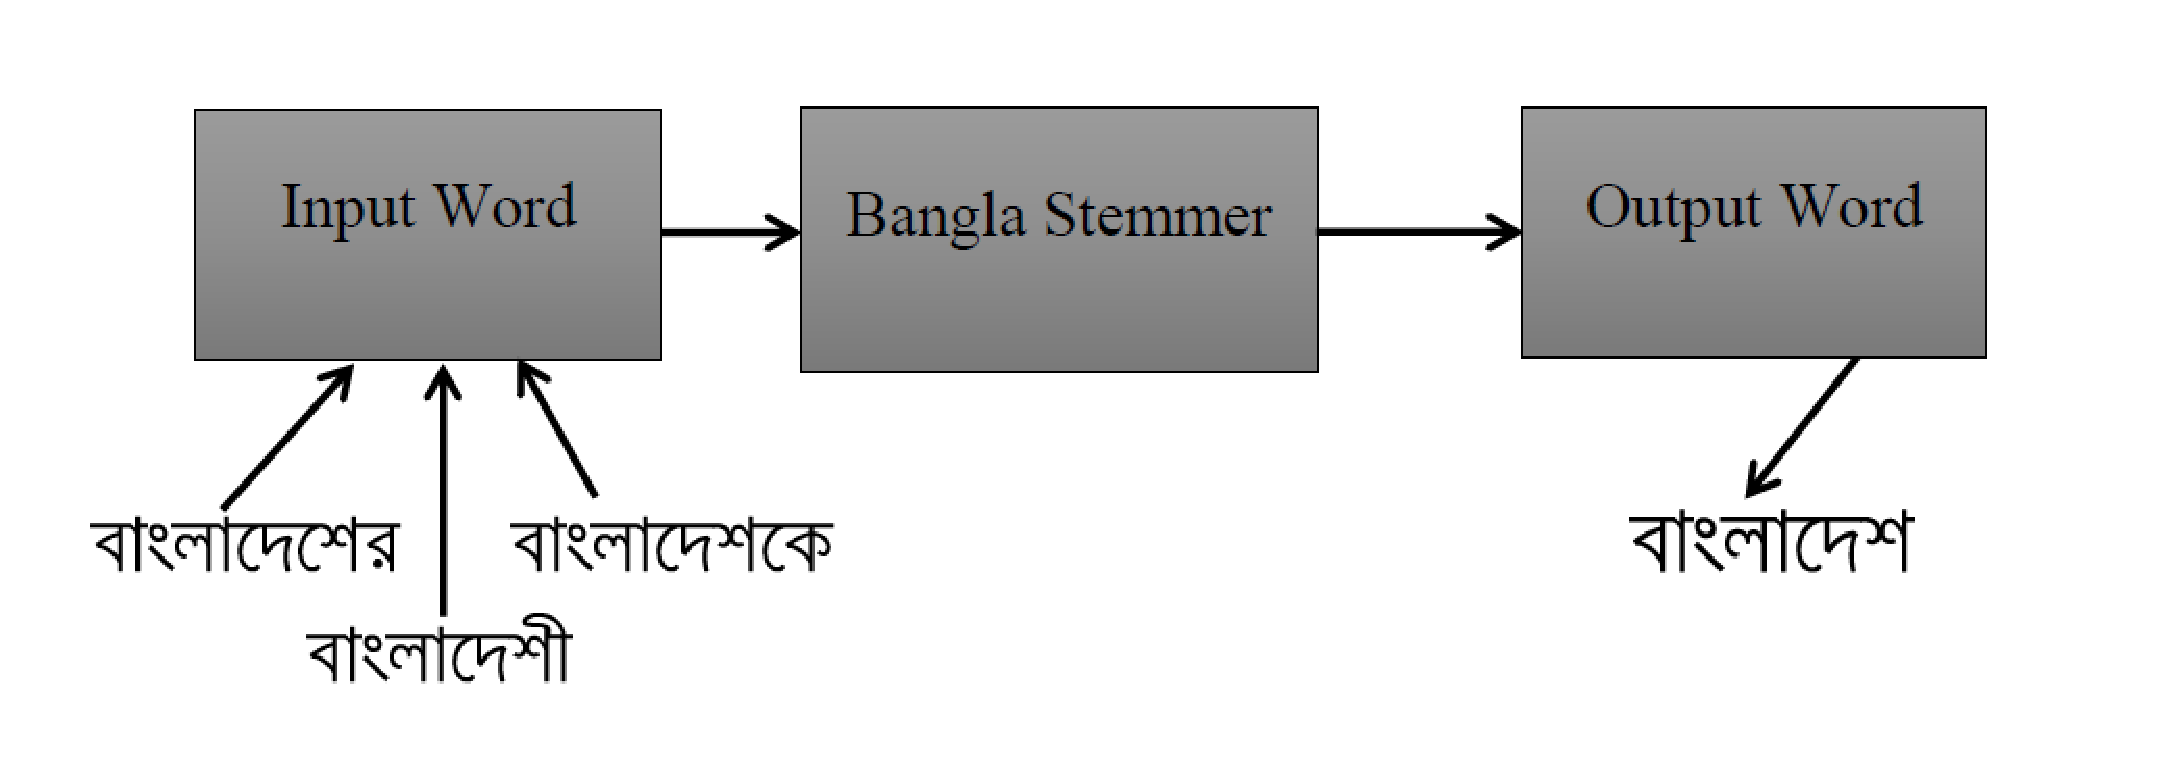
\includegraphics[width=.65\textwidth]{figure/four.eps}
	\caption{Stemming processing}
	\label{Figure:stemm}
\end{figure*}


\section{Cosine Similarity}

The query matches with relevent documents. If exists, find out the relevent documents and give them a scores using query term’s IDF multiplying with weight. Then sort the values and rank the documents.

Example:
There are three documents.\\
	D1: {\unicodefont আমি  বাংলাদেশকে ভালবাসি । বাংলাদেশ নদীমাতৃক দেশ।} \\
	D2: {\unicodefont আমি বাংলাদেশের নাগরিক । কিন্তু বাংলাদেশের সকল  নাগরিক তাদের মোলিক অধিকার পায় না। }\\
	D3: {\unicodefont বাংলাদেশ উন্নয়নশীল দেশ। এখনো উন্নয়নের দিক থেকে পিছিয়ে আছে বাংলাদেশ ।  }\\
	
	%{\unicodefont বাংলাদেশের নাগরিক হিসেবে বাংলাদেশের উন্নতি চাই।}
Input Query: {\unicodefont বাংলাদেশের নাগরিক হিসেবে বাংলাদেশের উন্নতি চাই।}\\

\(Cosine(document , query)  = (document . query) / |document vt | |query vt|\)\\


Now in table \ref{tab:Scoring} we can see the scores after doing the all process.

\begin{table*}[htp]	
\centering

\caption{Scoring Each Document  }
\vspace{0.5cm}
\begin{tabular}{|c|c|c|} 
\hline

	\textbf{Document Id }& \textbf{Documents} & \textbf{Scores} \\ \hline
 1 & D1 &	0.145   \\ \hline
 2 & D2 & 0.543   \\ \hline
 3 & D3  &0.345   \\ \hline


\end{tabular}
\label{tab:Scoring}
\end{table*}

After sorting scores, we get the ranked documents and we can see that in table \ref{tab:Rank}.


\begin{table*}[htp]	
\centering
\caption{Rank Documents  }
\vspace{0.5cm}
\begin{tabular}{|c|c|c|} 
\hline

\textbf{Document Id}  & \textbf{Documents} & \textbf{Scores} \\ \hline
 2 & D2 &	0.543   \\ \hline
 3 & D3 & 0.345   \\ \hline
 1 & D1 &0.145  \\ \hline


\end{tabular}
\label{tab:Rank}
\end{table*}


\section{Main Approaches}

When the preprocessing is completed, then our main process focuses on the analysis of the processed output by our own developed tools for Bangla document ranking. Our main approach are includes to generating term frequency vector, assigning cosine similarity to the corresponding document are known as document scoring. Then sorting the scores, we rank the documents. In figure \ref{Figure:graphical} shows the overall graphical view of our proposed system.

\begin{figure*}[htp]
	\centering
		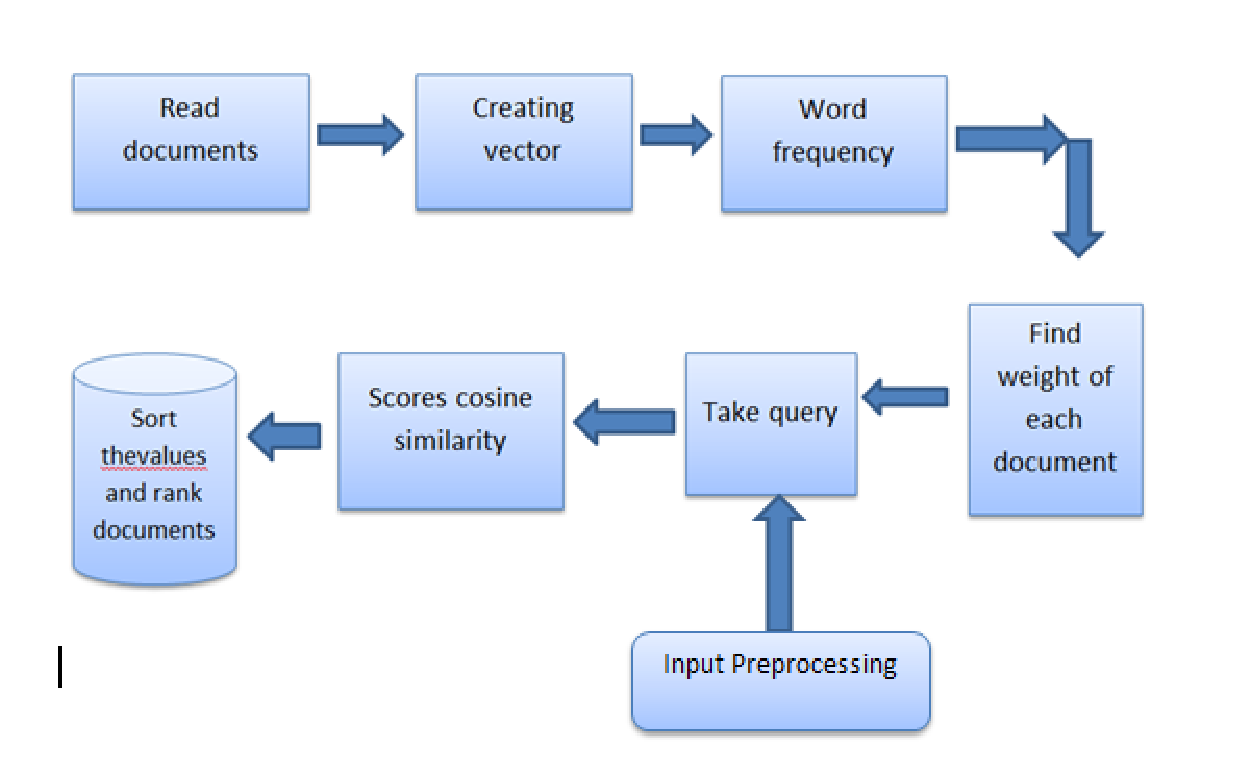
\includegraphics[width=.65\textwidth]{figure/five.eps}
	\caption{Overall graphical view of our proposed system}
	\label{Figure:graphical}
\end{figure*}


\chapter{Implementation}
\label{Ch_Chapter4}

Implementation is the process where we can see how our system works steps by steps.

\section{Bangla Corpus}

Bangla language contains huge range of vocabulary which makes the language variegated in the world. Here, we develop a dictionary data set where 30 documents are used. In this system, we use the dictionary several times. It has two main reasons to access this dictionary.  First one is to check a word which is rooted or not and second one is to get the associated POS tag for a word.

\section{Bangla Stemming}

Stemming is an operation that splits a word into its constituent root part and affix without doing complete morphological analysis. Terms with common stems tend to have similar meaning, which makes stemming an attractive option to increase the performance of news categorization task, where morphological analysis would be too computationally expensive. Another advantage of stemming is that it drastically reduce the vocabulary size of highly inflected languages corpus like Bangla.
The algorithm of using bangla stemmer


\begin{algorithm}[H]
 %\KwData{this text}
 %\KwResult{how to write algorithm with \LaTeX2e }
 %initialization\;
 \While{each word 2 document}{
  dictionary-checkers(word)\;
  \eIf{word 2 dictionary}{
   stem=word\;
   %current section becomes this one\;
   }{
   stem1=stemming(word)\;
	\eIf{stem1 2 dictionary}{stem=stem1}
	{stem=stemming(stem1)}
  }
	}
 
 \caption{bangla-stemmer (word)}

\end{algorithm}


\section{Bangla Stop Words}

Statistical analysis through the documents showed that some words have quite low frequency, while some others act just the opposite. The common characteristic of these words is that they carry no significant information and used just because of grammar. This set of words are usually known as stop words.  In the resulting stop word list, there were thus a large number of pronouns, articles, prepositions, and conjunctions. As in various English stop-word lists, there
were also some verbal forms. When using, this stop word list, the vocabulary size reduced significantly.


\section{Term Weighting}

Term Weighting of documents can be evaluated by measuring the Term Frequency (TF) and Inverse Document Frequency (IDF). These are the statistical measurement of weight that is
intended to determine the importance of a word for a document in a corpus. It can be used for stop-word filtering. This is the combine definition of Normalized Term Frequency and Inverse Document Frequency.


\subsection{TF}

Term Frequency measures how frequently a word occurs in a document. Different document varies in length. Therefore, a word can be occurring more times in a larger document than shorter. Thus, the raw frequency of a word is divided by the length of the document.

\begin{equation}
tf(t,d) = \frac{f(t,d)}{length of d}
\label{eq:tf}
\end{equation}


%\(tf(t,d) = \frac{f(t,d)}{length of d}\)

here f(t,d) is the raw frequency of word t in document d. Using equation \ref{eq:tf} ,term frequency can be defined.

\subsection{IDF}

Inverse Document Frequency measures the importance of a word within a document. TF provides same importance for every word, where IDF provides less weight to the frequent word and high weight to the rare word.

\begin{equation}
idf(t) = log(N/DF)
\label{eq:idf1}
\end{equation}

%\(idf(t) = log(N/DF)\)

Using equation \ref{eq:idf1}, the idf can be measured.

The TF-IDF weighting scheme sets a weight to a word t in document d,which is shown in equation \ref{eq:idf2}


\begin{equation}
tf -idf(t ,d) = tf (t ,d) * idf(t)
\label{eq:idf2}
\end{equation}

%\(tf -idf(t ,d) = tf (t ,d) * idf(t)\)

The weight of a word t in document d is highest when t occurs many times in a small number of document, and lower when t occurs a very few times in a document or occurs in many documents of the corpus.


\section{Cosine Similarity between query and document}

The similarity measures comparing between document vector and query vector. Though the angle between two vectors considered (0 to 90), than the similarity lies between 1 to 0.

\begin{equation}
Similarity = \cos\theta = \frac{\overrightarrow{A}.\overrightarrow{B}}{|\overrightarrow{A}||\overrightarrow{B}|}
\label{eq:cosine}
\end{equation}

%\(\)

The equation \ref{eq:cosine} is used for defining similarity.



\chapter{Conclusions and Future Scopes}
\label{Ch_Conclusion}

\section{Conclusion}

In Bangla document ranking, the term frequency and cosine similarity perform the utmost level of accuracy (88.10\%) than any other existing methods. The model we’ve described treats all documents on an equal footing. In addition to, this is the extraction based ranking system, is not real time ranking formation. In the typical web search setting it is important to users that the most relevant documents are top-ranked given the large number of potentially relevant documents. For each term in the dictionary, it’s straightforward to pre compute the top 1,000(say) documents for that term. Then for a given multi-term query it’s pretty likely that the top search results will come from one of the pre-computed lists of top documents for the terms in the query.

\section{Future Scopes}

The problem is that it computes the cosine similarity for every single document in the corpus. In future, ideas that are used in other methods, will be used together with the proposed approaches to improve the performance of the ranking system. We will compare our method with other methods.

%
\fancyhead[RE,LO]{{\footnotesize\rightmark} }


\renewcommand{\headrulewidth}{0.5pt}
%
\bibliographystyle{IEEEtran}
\switchchapter{fake} 
\addcontentsline{toc}{chapter}{Bibliography}
\bibliography{reference}
%\bibliography{BibTex}
%
\fancyhead[RE,LO]{{\footnotesize\rightmark} }
\renewcommand{\headrulewidth}{0.5pt}
%
\appendix 
\titlecontents{chapter}[6pc] 
  {\bfseries} 
  {\contentslabel[\appendixname\ \thecontentslabel]{6pc}} 
  {}{\hfill\contentspage} 
%
%\include{Acronyms}
%\include{Notations}
%\fancyhead[RE,LO]{\footnotesize{LIST OF PUBLICATIONS} \hspace{0.5em} {\footnotesize\rightmark} }
\renewcommand{\headrulewidth}{0.5pt}
%
\chapter{List of Publications}
\begin{center}
\textbf{\Large \underline {International Journal Papers}} \\
\end{center}
\begin{enumerate}
%
%\item \textbf{Sajal Halder} and Young-Koo Lee. \textit{Supergrpah based Periodic Behaviors Mining in Dynamic Networks}. In submission.

\item  \textbf{Sajal Halder}, Yongkoo Han, A. M. Jehad Sarkar and Young-Koo Lee. \textit{An Entertainment Recommendation System using the Dynamics of User Behavior over Time}. Decision in process in the Journal of Systems and Software.

\item	Md. Rezaul Karim, \textbf{Sajal Halder} , Byeong-Soo Jeong, and Ho-Jin Choi. \textit{Efficient Mining Frequently Correlated, Associated-correlated and Independent Patterns Synchronously by Removing Null Transactions}. Human Centric Technology and Service in Smart Space, pages 93-103, 2012. 

%\vspace{0.1in}
\item \textbf{Sajal Halder}, A. M. Jehad Sarkar and Young-Koo Lee. \textit{A synthetic trajectory-based moving objects generator}. Under review  in International Journal of Artificial Intelligence Tools.

\item \textbf{Sajal Halder}, Md. Mostofa Kamal Rasel, Yongkoo Han, and Young-Koo Lee. \textit{Mining Spatiotemporal Moving Objects Swarm}. Under review in Kyung Hee University Journal..

\pagebreak


%
\begin{center}
\textbf{\Large \underline{International Conference Papers}} 
\end{center}

\item Sajal Halder, Yongkoo Han and Young-Koo Lee. \textit{Discovering Periodic Patterns using Supergraph in Dynamic Networks}. Accepted in 5th International Conference on Data Mining and Intelligent Information Technology Applications (ICMIA),Jun 18-20, South Korea, 2013.

%
\item Sajal Halder, A. M. Jehad Sarkar and Young-Koo Lee. \textit{Movie Recommendation System Based on Movie Swarm}. Second International Conference on Cloud and Green Computing (CGC), China, Nov 1-3, 2012.
%\vspace{0.1in} 
\item Sajal Halder, Md. Samiullah, A. M. Jehad Sarkar and Young-Koo Lee. \textit{MovieSwarm: Information Mining technique for Movie Recommendation System}. In the 7th International Conference on Electrical and Computer Engineering (ICECE), Bangladesh, Dec 20-22, 2012.


\begin{center}
\textbf{\Large \underline{Thesis/Project Works}} 
\end{center}

\item Sajal Halder, Uzzal Kumar Dutta, Uttam Kumer Biswas and Asish Kumar Biswas ``Classification of Multiple Protein Sequences by means of Irredundant Patterns'', B.Sc. Final Year Project, Department of Computer Science and Engineering (CSE), University of Dhaka (DU), Bangladesh, February, 2011.
%
%\item Sabbir Ahmed, Md. Obaidur Rahman, Saifur Rahman Pir, M. A. Mottalib and Md. Saiful Islam; \textquotedblleft A New Approach towards the Development of English to Bangla Machine Translation System\textquotedblright, \textit{B.Sc. Engg. Final Year Project, Department of Computer Science $\&$ Information Technology (CIT), Islamic University of Technology (IUT)}, Bangladesh, September, 2003
%
\end{enumerate}
%

%
\end{document}
%
